\documentclass{article}
\usepackage{sivaNMSC}
\chead{Assignment $1$}

\begin{document}
	\begin{enumerate}
		\item
		We build a computer, where the real numbers are represented using $5$ digits as explained below:
		\begin{center}
		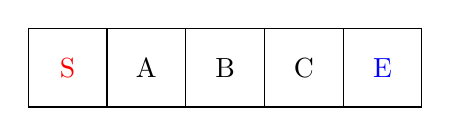
\begin{tikzpicture}
			\draw (0,0) grid (5,1);
			\node at (0.5,0.5) {\color{red}S};
			\node at (1.5,0.5) {A};
			\node at (2.5,0.5) {B};
			\node at (3.5,0.5) {C};
			\node at (4.5,0.5) {\color{blue}E};
		\end{tikzpicture}
		\end{center}
		where
		\begin{itemize}
			\item
			{\color{red}S} is the sign bit; $0$ for positive and $1$ for negative
			\item
			A,B,C: First three significant digits in decimal expansion with the decimal point occuring between A and B
			\item
			E is the exponent in base $10$ with a bias of $5$
			\item
			All digits after the third significant digit are chopped off
			\item
			$+0$ is represented by setting $S=0$ and $A=0$ (B,C,E) can be anything
			\item
			$-0$ is represented by setting $S=1$ and $A=0$ (B,C,E) can be anything
			\item
			$+\infty$ is represented by $S=0$, $A=B=C=E=9$
			\item
			$+\infty$ is represented by $S=1$, $A=B=C=E=9$
			\item
			Not A Number is represented by setting $S$ other than $0$ and $1$.
		\end{itemize}
		For example, the number $\pi=3.14159\ldots$ is represented as follows. Chopping off after the third significant digit, we have $\pi = +3.14 \times 10^0$. Hence, the represention of $\pi$ in our system is:
		\begin{center}
		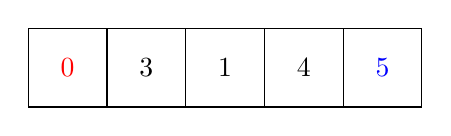
\begin{tikzpicture}
			\draw (0,0) grid (5,1);
			\node at (0.5,0.5) {\color{red}0};
			\node at (1.5,0.5) {3};
			\node at (2.5,0.5) {1};
			\node at (3.5,0.5) {4};
			\node at (4.5,0.5) {\color{blue}5};
		\end{tikzpicture}
		\end{center}
		The number $-0.001259$ is represented as follows. Chopping off after the third significant digit, we have the number as $-1.25 \times 10^{-3}$. Hence, the represention in our system is:
		\begin{center}
		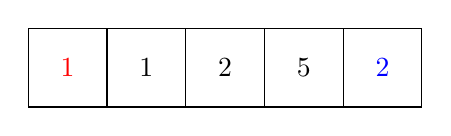
\begin{tikzpicture}
			\draw (0,0) grid (5,1);
			\node at (0.5,0.5) {\color{red}1};
			\node at (1.5,0.5) {1};
			\node at (2.5,0.5) {2};
			\node at (3.5,0.5) {5};
			\node at (4.5,0.5) {\color{blue}2};
		\end{tikzpicture}
		\end{center}
		Answer the following questions:
		\begin{enumerate}
			\item
			How many non-zero floating point numbers (from now on abbreviated as FPN) can be represented by our machine (both positive and negative)?
			\item
			How many FPNs are in the following intervals?
			\begin{itemize}
				\item
				$(9,10)$
				\item
				$(10,11)$
				\item
				$(0,1)$
			\end{itemize}
			\item
			Identify the smallest positive and largest positive FPN on this machine.
			\item
			Identify the machine precision.
			\item
			What is the smallest positive integer not representable exactly on this machine?
			\item
			Consider the recurrence:
			$$a_{n+1}=5a_n-4a_{n-1}$$
			with $a_1=a_2=2.93$. Note that $a_1$, $a_2$, $5$ and $4$ are exactly represnted on our machine. Compute $a_n$ for $n \in \{3,4,\ldots,10\}$ in our machine (Work out the values by hand). Note that at each step in the recurrence $5a_n$ and $4a_{n-1}$ will be both chopped down to the first three significant digits before the subtraction is performed.
		\end{enumerate}
		\item
		Consider the following integral:
		$$I_n = \dint_0^1 x^{2n} \sin\bkt{\pi x} dx$$
		\begin{itemize}
			\item
			Obtain a recurrence relation for $I_n$ in terms of $I_{n-1}$. (HINT: Integration by parts).
			\item
			Evaluate $I_0$.
			\item
			Use the recurrence above to obtain $I_n$ for $n \in \{1,2,3,\ldots,15\}$ in Python.
			\item
			Use the built-in quadrature function in Python to obtain $I_n$ for $n \in \{1,2,3,\ldots,15\}$.
			\item
			Explain your observation.
			\item
			Rewrite the equations in matrix form, i.e.,
			$$Ay = b$$
			\item
			Plot the condition number of the matrix $A$ as a function of $n$.
			\item
			Comment on how the condition number scales with $n$.
			\item
			Comment on the relationship of the condition number and accuracy of the solution $I_n$ obtained.
		\end{itemize}
		\item
		Show that if the parabolic run-out conditions are used for the cubic spline interpolation, then the interpolating polynomials in the first and last intervals are indeed parabolas.
		\item
		A slightly easier spline interpolation is the so-called quadratic spline. Interpolation is carried out by piecewise quadratics.
		\begin{itemize}
			\item
			What are the suitable joint conditions for quadratic spline?
			\item
			Show how the coefficients of this spline are obtained.
			\item
			What are the suitable end conditions?
			\item
			Compare the required computational efforts for quadratic and cubic spline.
			\item
			Write a Python code for interpolating the Runge function $f(x) = \dfrac1{1+25x^2}$ at equi-spaced nodes using a quadratic spline.
		\end{itemize}
	\end{enumerate}
\end{document}